\chapter{Extensive Form Games}

\section{Formalization: Tree and Play}

An extensive form game models sequential interactions. It is represented by a \textbf{game tree} $T$.

\subsection{The notion of "Play"}
Although intuitive, the distinction between strategy and play is fundamental.
\begin{definition}[Play]
A \textbf{play} is a complete path starting from the root of the tree and ending at a leaf (terminal node).
\end{definition}

\begin{proposition}
Given a pure strategy profile $x = (x_1, \dots, x_n)$, this generates a \textbf{unique play} $\pi(x)$.
However, several different strategy profiles can generate the same play (if their differences are only at unreached nodes).
\end{proposition}

\section{Game Tree Representation}

A game tree contains:
\begin{itemize}
    \item \textbf{Decision nodes:} Identify which player is to move.
    \item \textbf{Branches:} Possible actions at each node.
    \item \textbf{Leaves:} Final outcomes and payoffs.
\end{itemize}

\subsection{Nice Extensive Form Games}
\begin{definition}
A "Nice Extensive Form Game" is an extensive form game satisfying:
\begin{enumerate}
    \item A \textbf{finite} tree (finite horizon, finite nodes, finite edges).
    \item At each node (except terminal ones), there is a \textbf{unique} designated player.
    \item At terminal nodes, there are real payoff vectors (one for each player).
\end{enumerate}
\end{definition}

\begin{exemple}[3-Player Game - Course Diagram]
\begin{center}
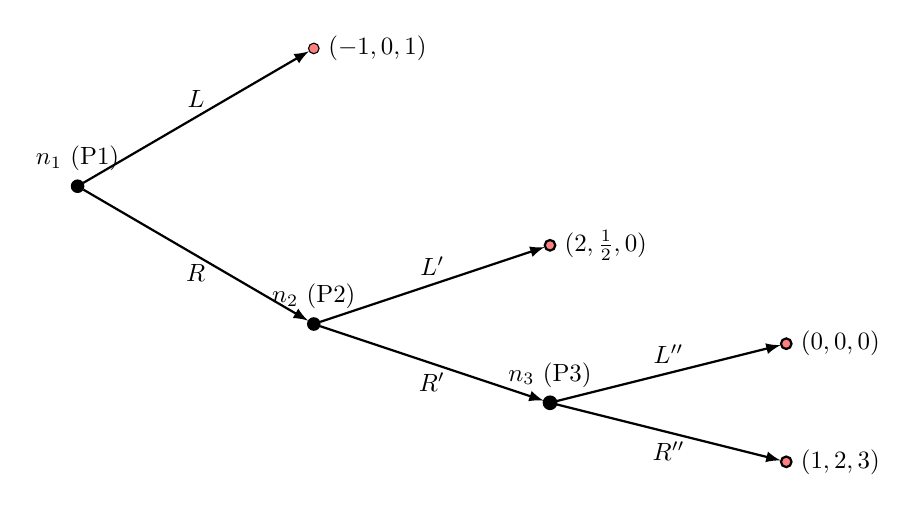
\begin{tikzpicture}[
    grow=right,
    level 1/.style={sibling distance=3.5cm,level distance=3cm},
    level 2/.style={sibling distance=2cm, level distance=3cm},
    level 3/.style={sibling distance=1.5cm, level distance=3cm},
    edge from parent/.style={draw, -latex, thick},
    every node/.style={scale=0.9},
    player/.style={circle, draw, fill=black, inner sep=1.5pt, minimum size=5pt},
    term/.style={circle, draw, fill=red!50, inner sep=1.5pt}
]
% Root Player 1
\node[player, label=above:{$n_1$ (P1)}] (root) {}
    child {
        node[player, label=above:{$n_2$ (P2)}] (n2) {}
        child {
            node[player, label=above:{$n_3$ (P3)}] (n3) {}
             child {
                node[term, label=right:{$(1,2,3)$}] {}
                edge from parent node[below] {$R''$}
            }
            child {
                node[term, label=right:{$(0,0,0)$}] {}
                edge from parent node[above] {$L''$}
            }
            edge from parent node[below] {$R'$}
        }
        child {
            node[term, label=right:{$(2, \frac{1}{2}, 0)$}] {}
            edge from parent node[above] {$L'$}
        }
        edge from parent node[below] {$R$}
    }
    child {
        node[term, label=right:{$(-1, 0, 1)$}] {}
        edge from parent node[above] {$L$}
    };
\end{tikzpicture}
\end{center}
\textbf{Legend:} Players in black ($1, 2, 3$), terminal nodes in red.
The story: Player 1 chooses $L$ or $R$. If they choose $L$, the game ends. If they choose $R$, it's Player 2's turn, etc.
\end{exemple}

\begin{exemple}[Market Entry Game]
Firm A (Entrant) decides to Enter (E) or Not (N). If it enters, Firm B (Incumbent) decides to Fight (B) or Accept (A).

\begin{center}
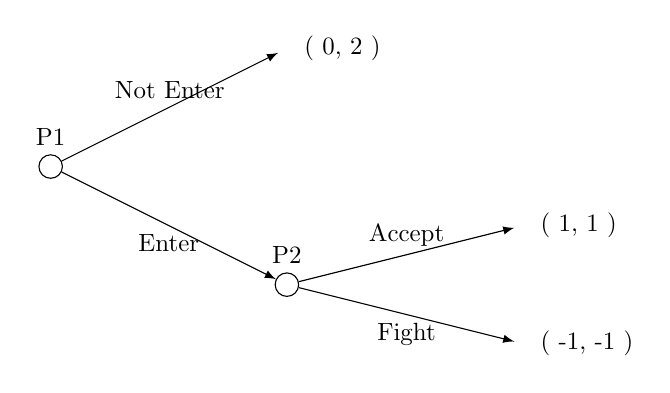
\begin{tikzpicture}[
    grow=right,
    level 1/.style={sibling distance=3cm,level distance=3cm},
    level 2/.style={sibling distance=1.5cm, level distance=3cm},
    edge from parent/.style={draw, -latex},
    every node/.style={scale=0.9}
]
\node[circle, draw, label=above:P1] (root) {}
    child {
        node[circle, draw, label=above:P2] (n1) {}
        child {
            node[label=right:{( -1, -1 )}] {}
            edge from parent node[below] {Fight}
        }
        child {
            node[label=right:{( 1, 1 )}] {}
            edge from parent node[above] {Accept}
        }
        edge from parent node[below] {Enter}
    }
    child {
        node[label=right:{( 0, 2 )}] {}
        edge from parent node[above] {Not Enter}
    };
\end{tikzpicture}
\end{center}
\end{exemple}

\section{Information and Strategies}

\subsection{Perfect vs Imperfect Information}
\begin{itemize}
    \item \textbf{Perfect Information:} Each player knows the complete history of the game (all nodes are singletons).
    \item \textbf{Imperfect Information:} Some nodes are grouped into \textbf{information sets}. The player knows they are in the set, but not at which specific node.
\end{itemize}

\begin{center}
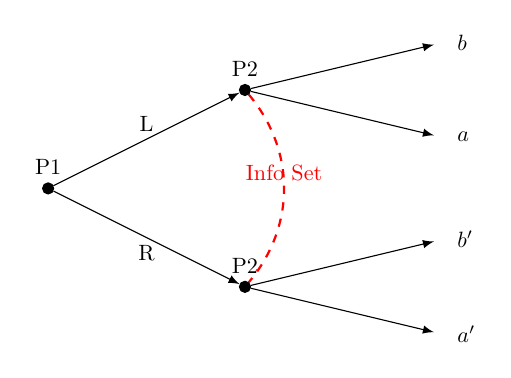
\begin{tikzpicture}[
    grow=right,
    level 1/.style={sibling distance=2.5cm,level distance=2.5cm},
    level 2/.style={sibling distance=1.2cm, level distance=2.5cm},
    edge from parent/.style={draw, -latex},
    every node/.style={scale=0.8},
    player/.style={circle, draw, fill=black, inner sep=1.5pt, minimum size=5pt}
]
% Root P1
\node[player, label=above:P1] (root) {}
    child {
        node[player, label=above:P2] (n2) {}
        child { node[label=right:{$a'$}] {} edge from parent }
        child { node[label=right:{$b'$}] {} edge from parent }
        edge from parent node[below] {R}
    }
    child {
        node[player, label=above:P2] (n1) {}
        child { node[label=right:{$a$}] {} edge from parent }
        child { node[label=right:{$b$}] {} edge from parent }
        edge from parent node[above] {L}
    };
% Information set (dashed ellipse connecting n1 and n2)
\draw[dashed, thick, red] (n1) to[bend left=40] node[midway, above, red] {Info Set} (n2);
\end{tikzpicture}
\captionof{figure}{Information Set: P2 does not know if P1 played L or R.}
\end{center}

\subsection{Condensed Strategy Notation}
A major distinction of the course:
\begin{definition}[Strategy]
A \textbf{strategy} is a \textbf{complete} and \textbf{exhaustive} plan of action: it specifies an action for \textit{every} information set where the player is called to play, \textbf{even those that will never be reached} if the strategy is followed.
\end{definition}

\subsection{Normal Form associated with Extensive Form}
\begin{definition}
To any extensive form game $\Gamma$, we can associate a normal form game (matrix) defined by:
\begin{itemize}
    \item The same players.
    \item Strategies defined as complete action plans (e.g., $W'N'$).
    \item Payoffs determined by the unique play generated by each strategy profile.
\end{itemize}
\end{definition}

\begin{exemple}[ "Nuclear Weapon" Game - Course Example]
\textbf{1. Game Tree ($\Gamma$):}
Player 1 (P1) chooses Nuclear Weapon ($W$) or Not ($N$). Player 2 (P2) reacts.
\begin{center}
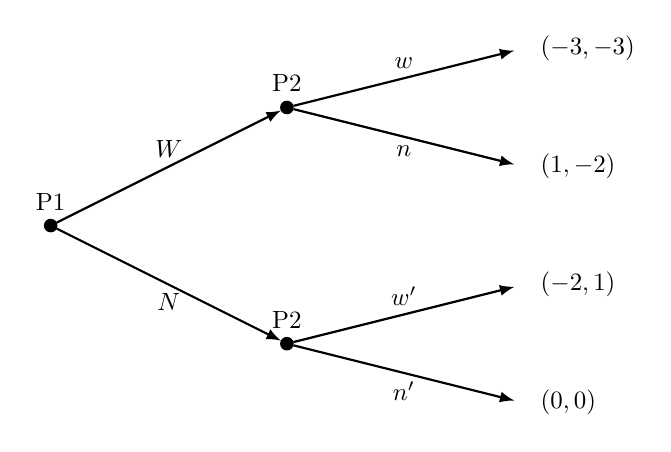
\begin{tikzpicture}[
    grow=right,
    level 1/.style={sibling distance=3cm,level distance=3cm},
    level 2/.style={sibling distance=1.5cm, level distance=3cm},
    edge from parent/.style={draw, -latex, thick},
    every node/.style={scale=0.9},
    player/.style={circle, draw, fill=black, inner sep=1.5pt, minimum size=5pt}
]
\node[player, label=above:P1] (root) {}
    child {
        node[player, label=above:P2] (n2) {}
        child {
            node[label=right:{$(0,0)$}] {}
            edge from parent node[below] {$n'$}
        }
        child {
            node[label=right:{$(-2,1)$}] {}
            edge from parent node[above] {$w'$}
        }
        edge from parent node[below] {$N$}
    }
    child {
        node[player, label=above:P2] (n1) {}
        child {
            node[label=right:{$(1,-2)$}] {}
            edge from parent node[below] {$n$}
        }
        child {
            node[label=right:{$(-3,-3)$}] {}
            edge from parent node[above] {$w$}
        }
        edge from parent node[above] {$W$}
    };
\end{tikzpicture}
\end{center}
\textit{Note: The notations $w, n$ (left) and $w', n'$ (right) for P2 allow constructing their strategies.}

\textbf{2. Strategies:}
\begin{itemize}
    \item P1: $\{W, N\}$
    \item P2: $\{ww', wn', nw', nn'\}$ (Often denoted $W'W', W'N'$ etc. in notes).
    Example: $wn'$ means "I play w if P1 plays W, and I play n' if P1 plays N".
\end{itemize}

\textbf{3. Payoff Matrix (Normal Form):}
Each cell corresponds to the payoff of the reached leaf.
$$
\begin{array}{c|c|c|c|c}
P1 \setminus P2 & ww' & wn' & nw' & nn' \\
\hline
W & (-3,-3) & (-3,-3) & (1,-2) & (1,-2) \\
\hline
N & (-2,1) & (0,0) & (-2,1) & (0,0) \\
\end{array}
$$
\textit{Explanation:} If P1 plays $W$ and P2 plays $wn'$, the game goes to $W$ then to $w$. Payoff $(-3,-3)$.
\end{exemple}


\section{Backward Induction and Credibility}

\subsection{Backward Induction}
To solve a finite game with perfect information, we reason backwards:
\begin{enumerate}
    \item Focus on the last decision nodes.
    \item The player chooses the action maximizing their payoff.
    \item Replace the subgame with these payoffs (we "prune" the tree).
    \item Move up to the root.
\end{enumerate}

\begin{theoreme}
The backward induction algorithm determines a \textbf{Subgame Perfect Nash Equilibrium (SPE)}.
\end{theoreme}

\begin{definition}[Subgame Perfect Equilibrium - SPE]
A strategy profile is a \textbf{Subgame Perfect Equilibrium (SPE)} if it induces a Nash equilibrium in \textbf{every subgame} of the tree (including the whole game).
\end{definition}

\begin{exemple}[Exam: SPE vs Nash]
Consider the following game: P1 chooses $A$ or $D$ (payoff 2,2). If $A$, P2 chooses $l$ or $r$. If $l$, P1 chooses $L(4,2)$ or $R(1,0)$. If $r$, P1 chooses $L'(0,3)$ or $R'(3,1)$.
\begin{itemize}
    \item \textbf{Normal Form:} P1 has 4 strategies $\{AL, AR, DL, DR\}$. P2 has 2 $\{l, r\}$.
    \item \textbf{Nash Equilibria:} $(AL, r)$ (Payoff $0,3$), $(DL, l)$ (Payoff $2,2$), $(DR, l)$ (Payoff $2,2$).
    \item \textbf{Subgame Analysis (Induction):}
    \begin{enumerate}
        \item Subgame after $(A,l)$: P1 chooses $L$ (4 > 1).
        \item Subgame after $(A,r)$: P1 chooses $R'$ (3 > 0).
        \item P2 anticipates: if they play $l$, P1 plays $L$ (P2 payoff = 2). If they play $r$, P1 plays $R'$ (P2 payoff = 1). P2 chooses $l$.
        \item Root: P1 anticipates that $A$ leads to $L$ (payoff 4). $D$ leads to 2. P1 chooses $A$.
    \end{enumerate}
    \item \textbf{Conclusion:} The unique SPE is the path $(A, l, L)$ given by the complete strategies \textbf{(P1: $A, L, R'$; P2: $l$)}.
    \item \textbf{Analysis:} The Nash equilibrium $(DL, l)$ is not an SPE because it relies on the (implicit) threat that P1 would play poorly in the subgame $(A,r)$ (they would not play their best response).
\end{itemize}
\end{exemple}

\section{Practical Case: The Centipede Game}
...

\section{Exercises}
\subsection{Exercise "Tree and Matrix" (Handwritten Notes)}
Consider the following game: P1 chooses $a$ or $b$. P2 then chooses ($c,d$ if $a$; $c',d'$ if $b$).
\begin{center}
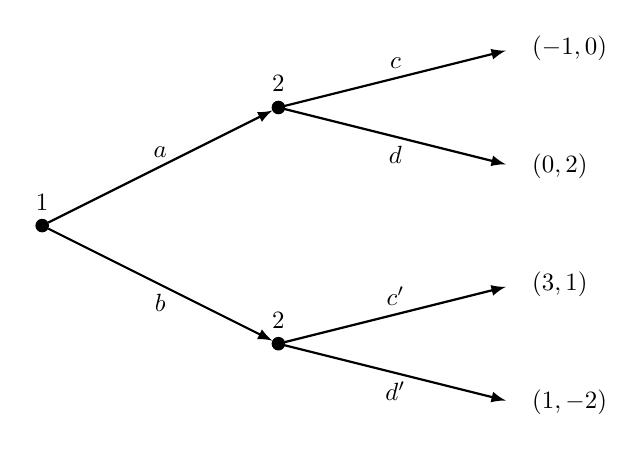
\begin{tikzpicture}[
    grow=right,
    level 1/.style={sibling distance=3cm,level distance=3cm},
    level 2/.style={sibling distance=1.5cm, level distance=3cm},
    edge from parent/.style={draw, -latex, thick},
    every node/.style={scale=0.9},
    player/.style={circle, draw, fill=black, inner sep=1.5pt, minimum size=5pt}
]
\node[player, label=above:1] (root) {}
    child {
        node[player, label=above:2] (n2) {}
        child {
            node[label=right:{$(1,-2)$}] {}
            edge from parent node[below] {$d'$}
        }
        child {
            node[label=right:{$(3,1)$}] {}
            edge from parent node[above] {$c'$}
        }
        edge from parent node[below] {$b$}
    }
    child {
        node[player, label=above:2] (n1) {}
        child {
            node[label=right:{$(0,2)$}] {}
            edge from parent node[below] {$d$}
        }
        child {
            node[label=right:{$(-1,0)$}] {}
            edge from parent node[above] {$c$}
        }
        edge from parent node[above] {$a$}
    };
\end{tikzpicture}
\end{center}
\textbf{Question:} Calculate the Nash Equilibria.
\\
\textbf{Answer:}
We construct the $2 \times 4$ matrix. P2 Strategies: $cc', cd', dc', dd'$.
$$
\begin{array}{c|c|c|c|c}
1 \setminus 2 & cc' & cd' & dc' & dd' \\
\hline
a & (-1,0) & (-1,0) & \mathbf{(0,2)} & \mathbf{(0,2)} \\
\hline
b & \mathbf{(3,1)} & (1,-2) & \mathbf{(3,1)} & (1,-2) \\
\end{array}
$$
\begin{itemize}
    \item If P1 plays $a$: P2 prefers $d$ (payoff 2) $\to$ columns $dc', dd'$. P1 responds $a$ or $b$? Compare $0$ and $3$. P1 prefers $b$. So no pure Nash on row $a$.
    \item If P1 plays $b$: P2 prefers $c'$ (payoff 1) $\to$ columns $cc', dc'$. P1 responds $b$ (3 vs -1 or 0).
    \item \textbf{Nash Equilibria:} $(b, cc')$ and $(b, dc')$.
    \item Equilibrium payoff: $(3,1)$.
\end{itemize}
\section{Backward Induction and Credibility}

\subsection{Backward Induction}
To solve a finite game with perfect information, we reason backwards:
\begin{enumerate}
    \item Focus on the last decision nodes.
    \item The player chooses the action maximizing their payoff.
    \item Replace the subgame with these payoffs (we "prune" the tree).
    \item Move up to the root.
\end{enumerate}

\begin{theoreme}
The backward induction algorithm determines a \textbf{Subgame Perfect Nash Equilibrium (SPE)}.
\end{theoreme}

\subsection{Non-Credible Threats}
Every SPE is a Nash equilibrium, but the converse is false.
\begin{itemize}
    \item A Nash equilibrium can rely on a "non-credible threat": the player promises a severe punishment (e.g., blowing themselves up) at a node that is not reached in equilibrium.
    \item Since the node is never reached, the threat costs nothing ("talk is cheap").
    \item The concept of SPE (and backward induction) eliminates these equilibria by demanding rationality \textbf{everywhere}, even off the equilibrium path.
\end{itemize}

\section{Practical Case: The Centipede Game}

\textbf{Description:}
Two players take turns. At each round, a player can "Stop" (taking the large pile, leaving little to the other), or "Pass" (to increase the global pot).
The game has a fixed end (e.g., 100 rounds).

\textbf{Paradox of Backward Induction:}
\begin{itemize}
    \item At the last round (100), the deciding player has an incentive to Stop to take the payoff.
    \item Anticipating this, at round 99, the other player has an incentive to Stop to avoid getting nothing at round 100.
    \item By induction, backward induction predicts that \textbf{the first player stops at the very first round}!
\end{itemize}
\textbf{Conclusion:} Although rational in the SPE sense, this result is sub-optimal (Pareto-inferior to cooperation) and rarely observed in practice.

\section{Exercises}
\begin{exercice}[Extensive Form Games]
\begin{itemize}
    \item Represent the Sequential Prisoner's Dilemma.
    \item Verify that in the entry game, the threat "Fight" is not credible if the cost of fighting is too high.
\end{itemize}

\paragraph{Solution:}
\begin{enumerate}
    \item \textbf{Sequential PD:}
    J1 plays (C or D). Then J2 plays (C or D) knowing J1's choice.
    
    \begin{center}
    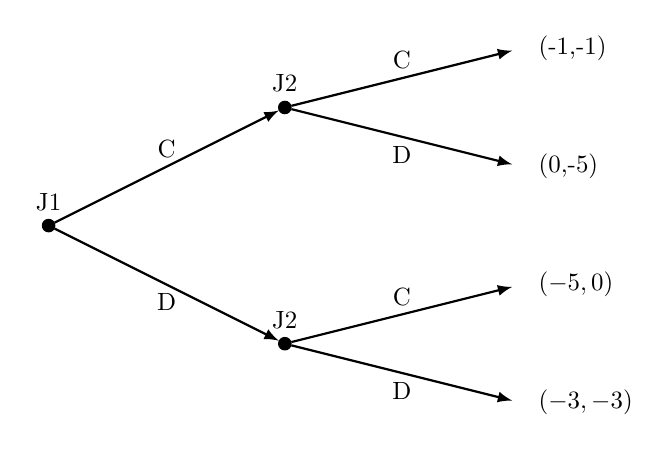
\begin{tikzpicture}[
        grow=right,
        level 1/.style={sibling distance=3cm,level distance=3cm},
        level 2/.style={sibling distance=1.5cm, level distance=3cm},
        edge from parent/.style={draw, -latex, thick},
        every node/.style={scale=0.9},
        player/.style={circle, draw, fill=black, inner sep=1.5pt, minimum size=5pt}
    ]
    \node[player, label=above:J1] (root) {}
        child {
            node[player, label=above:J2] (n2) {}
            child {
                node[label=right:{$(-3,-3)$}] {}
                edge from parent node[below] {D}
            }
            child {
                node[label=right:{$(-5,0)$}] {}
                edge from parent node[above] {C}
            }
            edge from parent node[below] {D}
        }
        child {
            node[player, label=above:J2] (n1) {}
            child {
                node[label=right:{(0,-5)}] {}
                edge from parent node[below] {D}
            }
            child {
                node[label=right:{(-1,-1)}] {}
                edge from parent node[above] {C}
            }
            edge from parent node[above] {C}
        };
    \end{tikzpicture}
    \end{center}
    
    \textbf{Backward Induction:}
    \begin{itemize}
        \item Top (if J1 plays C): J2 chooses D ($0 > -1$).
        \item Bottom (if J1 plays D): J2 chooses D ($-3 > -5$).
        \item J1 anticipates that C leads to $(0, -5)$ (for J2 it's payoff 0, for J1 it's -5?) \textit{Watch the payoffs (J1, J2)}.
        \item Let's verify payoffs:
        If (C, C) $\to (-1, -1)$.
        If (C, D) $\to (-5, 0)$. J2 gets 0.
        If (D, C) $\to (0, -5)$. J2 gets -5.
        If (D, D) $\to (-3, -3)$.
        \item \textbf{J2 Node (Top, after C):} J2 compares C (-1) and D (0). Chooses D.
        \item \textbf{J2 Node (Bottom, after D):} J2 compares C (-5) and D (-3). Chooses D.
        \item \textbf{J1 Root:} Anticipates (C $\to$ J2 plays D $\to$ J1 Payoff = -5) and (D $\to$ J2 plays D $\to$ f J1 Payoff = -3).
        \item J1 compares -5 and -3. Chooses D.
        \item \textbf{Result:} (D, D).
    \end{itemize}
    
    \item \textbf{Entry Game:}
    If the Entrant enters, the Incumbent has the choice between "Fight" (Payoffs: -1, -1) or "Accept" (Payoffs: 1, 1).
    Since $1 > -1$, the rational Incumbent will \textbf{always} choose to Accept.
    Any strategy where they threaten to fight is non-credible (does not withstand backward induction).
    The Entrant knows this, so they Enter (since $1 > 0$).
\end{enumerate}
\end{exercice}
